\documentclass[12pt]{beamer}
\title{Optimized Computation of the Q Factor in LAPACK}
\author{Johnathan Rhyne\\Advised by: Julien Langou}
\institute{University of Colorado Denver}
\usepackage{algorithm}
\usepackage{algpseudocode}
\usepackage{multicol}
\usepackage{environ}
\date{\today}

\newcommand{\customframefont}[1]{
\setbeamertemplate{itemize/enumerate body begin}{#1}
\setbeamertemplate{itemize/enumerate subbody begin}{#1}
}

\NewEnviron{framefont}[1]{
\customframefont{#1} % for itemize/enumerate
{#1 % For the text outside itemize/enumerate
\BODY
}
\customframefont{\normalsize}
}

\newcommand{\R}{\mathbb{R}}


%---------------%
% Abstract:     %
%---------------%
% Computing the Q Factor is an important operation for some applications and end users, so 
%  we aim to demonstrate new algorithms can speed up the performance of these operations for
%  end users. We implement existing algorithms 
%  originally developed by [insert authors here]. We see performance improvements on
%  the order of [insert rought value here] in comparison to the reference LAPACK 
%  computations and see similar performance in many cases as the optimized implementation
%  for AMD (AOCL). Using these schemes we not only see an improvement in execution time,
%  but lowers the memory footprint for the main driver algorithm.
%
%
%

\begin{document}
    \begin{frame}
        \titlepage
    \end{frame}
    % Table of contents. Can be helpful for navigating after the fact
    \begin{framefont}{\small}
    \begin{frame}
        \frametitle{Overview}
        \begin{multicols}{2}
            \tableofcontents
        \end{multicols}
    \end{frame}
    \end{framefont}
    \section{Preliminaries}
    \begin{frame}
        %
        %LAPACK stands for Linear Algebra PACKage, which provides a suite of routines to 
        %perform many linear algebra operations including but not limited to:
        %
        \frametitle{What is LAPACK}
        LAPACK provides interfaces for:
        \begin{enumerate}
            \item Matrix multiplication
            \item Solving linear systems of equations
            \item Factorizing matrices
        \end{enumerate}
        and more!
        %
        %We provide the interface and then set a baseline for chip vendors like INTEL and AMD to either package
        %or beat themselves.
        %
    \end{frame}
    \begin{frame}
        \frametitle{Notation}
        Throughout this presentation we will use the notation used by LAPACK. The first character determines what kind of numbers we are working with. Ex:
        \begin{itemize}
            \item DLACPY is the routine that copies double precision real numbers from one matrix to another
        \end{itemize}
        In this presentation, we will be restricting our discussion to only double precision real numbers,
        but there are analogous versions for single precision real, and both complex precisions.
    \end{frame}
    \begin{frame}
        \frametitle{Brief Linear Algebra Review}
        Householder reflectors are a way to to represent a matrix as a product of rank $1$ updates of the form
        $$
            \left(I - \tau_1 v_1v_1^\top\right)\cdots\left(I - \tau_k v_kv_k^\top\right) = I - VTV^\top
        $$
        Routines that use this\footnote{Collected by listing some functions found on the caller graph of DLARFT found \textcolor{blue}{\href{https://netlib.org/lapack/explore-html//d7/d0d/group__larft_ga20e5a4f351b3ca7d30078547e55884f5_ga20e5a4f351b3ca7d30078547e55884f5_icgraph_org.svg}{here}}}
        \begin{itemize}
            \item SVD *GESVD
            \item Hessenberg Reduction *GEBRD
            \item QR Factorization *GEQRF
        \end{itemize}
    \end{frame}
    \section{DORGQR Overview}
    \subsection{Existing Behavior}
    \begin{frame}
        \frametitle{LAPACK DORGQR}
        The algorithm for computing $Q$ is as follows
        \begin{algorithmic}
            \State Determine blocking parameter $nb$
            \State Initialize $Q$ as the $m\times m$ identity matrix
            \For{Each block of size $nb$ of $V$}
            \State Compute the $T$ factor
            \State Apply the block of reflectors to trailing columns of $Q$
            \State Apply the block of reflectors to the current block of columns of $Q$
            \EndFor
        \end{algorithmic}
    \end{frame}
    \subsection{Places for Optimization}
    \begin{frame}
        \frametitle{Places for Optimization}
        We have $4$ main places to look at to optimize this computation.
        \begin{enumerate}
            \item Computing $T$ (DLARFT)
            \item Applying to the trailing columns of $Q$ (DLARFB)
            \item Applying to the current window of $Q's$ columns (DORG2R)
            \item Take advantage of initializing $Q$ as $I_m$. (Main driver DORGQR)
        \end{enumerate}
    \end{frame}
    \section{Computation of T}
    \subsection{Existing Behavior}
    \begin{frame}
        \frametitle{LAPACK Implementation}
        % T upper triangular
        % Mention V is unit lower triangular in practice
        % At a high level, what the current dlarft does is compute T one column at a time.
        The algorithm for DLARFT is given by\footnote{Taken from the comments of DLARFT found \textcolor{blue}{\href{https://netlib.org/lapack/explore-html//dd/daa/dlarft_8f_source.html}{here}}\\\,}:
        \begin{algorithmic}
            \For{Each column of $V$}
                \State $T(1:i-1,i) = -\tau_i V(:,1:i-1)^\top * V(:,i)$
                \State $T(1:i-1,i) = T(1:i-1,1:i-1) * T(1:i-1,i)$
                \State $T(i,i) = \tau_i$
            \EndFor
        \end{algorithmic}

        % As we can see above, we are doing a bunch of matrix-vector operations. This leads to two kinds of improvements
        % The first being in restructuring the code to be recursive as this scheme can lead to performance gains
        % particularly when we have many more rows than columns
    \end{frame}
    \subsection{Recursive LARFT}
    \begin{frame}
        \frametitle{Recursive Implementation}
        % In order to motivate the recursive formulation, we notice that if we had a way to collect these
        % T values for the first l columns and the remaining, we want to do the following
        If we collect only some of the reflectors on the first and second half, we get
        \begin{align*}
            &\,(I - V_1T_{1,1}V_1^\top)(I - V_2T_{2,2}V_2^\top) \\
            &= I - V_1T_{1,1}V_1^\top - V_2T_{2,2}V_2^\top + V_1T_{1,1}V_1^\top V_2T_{2,2}V_2^\top
        \end{align*}
        Can be rewritten as:
        $$
            I - VTV^\top
        $$
        where:
        % Rewrite the T with indices
        % Write T out 
        % Then, if we define T_3 and V as follows, we can recover above!
        \begin{align*}
            T_{1,2} &= -T_{1,1}V_1^\top V_2T_{2,2} \\
            V &= \begin{bmatrix}
                V_1 \\ V_2
            \end{bmatrix}\\
            T &= \begin{bmatrix}
                T_{1,1} & T_{1,2} \\
                0       & T_{2,2}
            \end{bmatrix}
        \end{align*}
    \end{frame}
    \subsection{Matrix Operation LARFT}
    \begin{frame}
        \frametitle{Matrix Operation Implementation}
        % Add proper citation to these
        Based on the work done by Joffrain and et. al. \footnote{Accumulating Householder Transformations, Revisited} and Puglisi \footnote{Modification of the Householder method based on the compact wy representation}
        \\\,\\
        \begin{algorithmic}
            \State $T = V^\top V$ (Only upper triangular part)
            \State Scale the diagonal by $\frac{1}{2}$.
            \State $T = T^{-1}$.
        \end{algorithmic}
        \,\\\,\\
        For more details about why this works, see either Theorem 2 from Joffrain et. al. or the algorithm from Puglisi
    \end{frame}
    \subsection{Numerical Experiments}
    \begin{frame}
        \frametitle{Numerical Results}
        We ran the following tests on the Alderaan\footnote{Specifications for the cluster can be found 
        \textcolor{blue}{\href{https://ccm-docs.readthedocs.io/en/latest/alderaan\#hardware}{here}}\\\,} 
        cluster here at UC Denver\\
        % put pictures here of just the times.
        \begin{center}
        %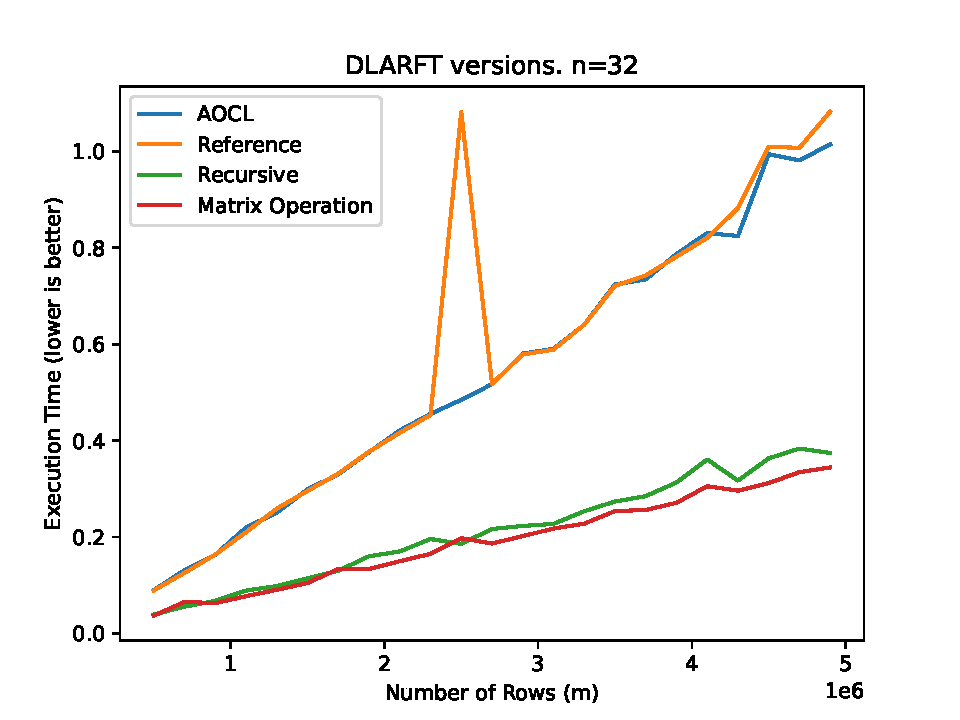
\includegraphics[width=.4\textwidth]{figs/dlarftNBTime.pdf}
        %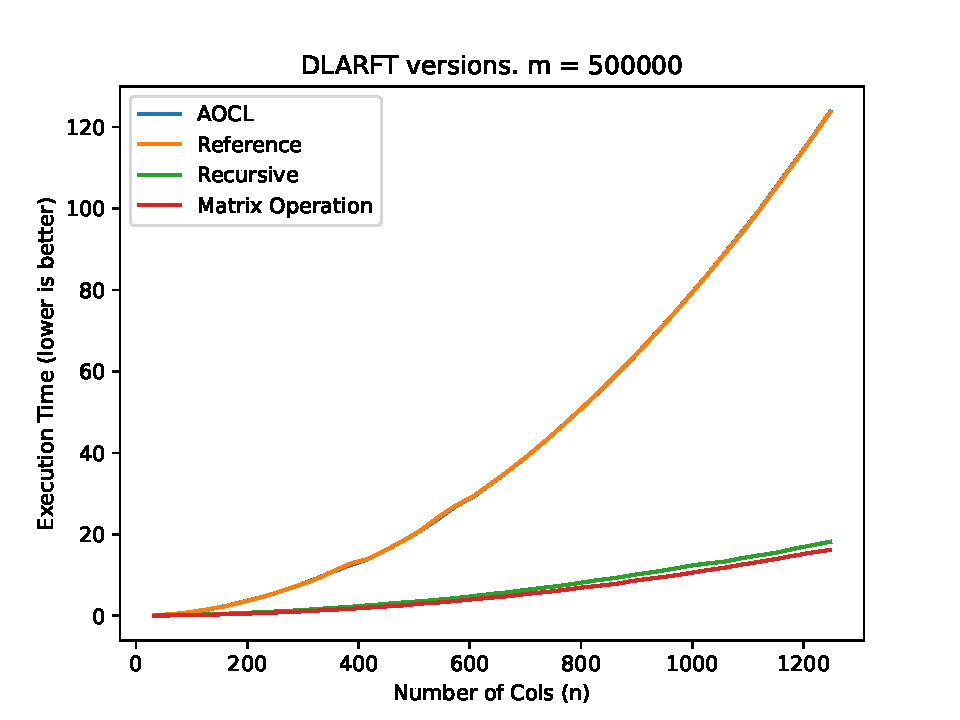
\includegraphics[width=.4\textwidth]{figs/dlarftNVaryTime.pdf}
        \end{center}
    \end{frame}
    \subsection{Computational Cost}
    %\begin{framefont}{\small}
    \begin{frame}
        \frametitle{Floating Point Operation Count}
        For these two different versions, we get the following computation cost for $V\in\R^{m\times n}$ and  $T\in\R^{n\times n}$
        \begin{align*}
            \text{DLARFT: }&\,  \frac{(n^2-1)(2m+n)}{6}\\
            \text{DLARFT\_REC: }&\, \frac{(n^2-1)(2m+n)}{6}\\
            \text{DLARFT\_MAT: }&\, \frac{6mn^2 + 6mn +4n^3 -9n^2 + 5n}{6}
        \end{align*}
        Even though we have more operations in the last version, we still see execution speeds on a similar level
        as recursive as we are using highly optimized BLAS routines.
    \end{frame}
    %\end{framefont}
    \section{DLARFB}
    \begin{frame}
        \frametitle{DLARFB Algorithm}
        Want to compute $C = HC$ where $H$ has the form
        $$
        H = I - VTV^\top
        $$
        And $C$ is any matrix of the proper shape. We break up $V$ and $C$ as follows
        $$
            V = \begin{bmatrix}
                V_1\\
                V_2
            \end{bmatrix} \qquad
            C = \begin{bmatrix}
                C_1\\
                C_2
            \end{bmatrix}
        $$
    \end{frame}
    \begin{frame}
        \frametitle{DLARFB Algorithm}
        By doing so, and doing some algebra, we get the following two updates we need to compute, which are
        \begin{align*}
            C_1 &= C_1 - V_1T\left(V_1^\top C_1 + V_2^\top C_2\right) \\
            C_2 &= C_2 - V_2T\left(V_1^\top C_1 + V_2^\top C_2\right)
        \end{align*}
    \end{frame}
    \subsection{Existing behavior}
    \begin{frame}
        \frametitle{Current Algorithm}
        %Assuming that $C$ is non-zero, we need an extra bit of memory of size $nb\times nb$.
        Reference LAPACK does the following with a workspace of size $nb\times nb$ denoted $W$\\\,\\
        \begin{algorithmic}
            \State $W = C_1^\top$
            \State $W = WV_1$
            \State $W = W + C_2^\top V_2$
            \State $W = WT^\top$
            \State $C_2 = C_2 - V_2W^\top$
            \State $W = WV_1^\top$
            \State $C_1 = C_1 - W^\top$
        \end{algorithmic}\,\\
        However, we get an extra bit of information that $C_1$ starts as the $0$ matrix, which is the correct
        size, so we can use that as a workspace instead!
    \end{frame}
    \subsection{New Behavior}
    \begin{frame}
        \frametitle{New algorithm}
        Taking advantage of the fact that for DORGQR, $C_1 = 0$, we have the following sequence of operations
        \begin{algorithmic}
            \State $C_1 = V_2^\top C_2$
            \State $C_1 = TC_1$
            \State $C_2 = C_2 - V_2C_1$
            \State $C_1 =     - V_1C_1$
        \end{algorithmic}
    \end{frame}
    \subsection{Flop Comparison}
    \begin{frame}
        \frametitle{Floating Point Operation Counts}
        For these two different versions, we get the following computation cost for $V\in\R^{m\times k}$, $T\in\R^{k\times k}$, and $C\in\R^{m\times n}$.\footnote{Note: In our actual loops, we grow $m$ and $n$, and $k$ is the blocking parameter usually just set to $32$.}
        \begin{align*}
            \text{DLARFB: }&\, 3nk^2 + 4(m-k)nk + nk\\
            \text{NEW\_DLARFB: }&\, 2nk^2 + 4(m-k)nk
        \end{align*}
        In addition to our memory savings, we also have a slight computation improvement. We don't see
        much of this benefit in computational cost in practice though. Note: we are also linear in $m$ and
        $n$, so we scale well when we treat $k$ as a constant blocking parameter.
    \end{frame}
    \section{DORG2R}
    \subsection{What it is supposed to do}
    \begin{frame}
        \frametitle{Unblocked version}
        DORG2R is specialized when we don't want to block at all. In general, this will be slower for most
        use cases, but is used in our blocked loop. So, we discuss the general behavior now.
    \end{frame}
    \subsection{Existing Behavior}
    \begin{frame}
        % Summary: This is just DORGQR with a blocksize of 1
        \frametitle{DORG2R algorithm inside DORGQR}
        \begin{algorithmic}
            \For{Each column of $V$ denoted $v_i$}
            \State Apply $I-\tau_iv_iv_i^\top$ to the trailing columns of $Q$
            \EndFor
        \end{algorithmic}
        This ends up being much slower as we are doing matrix vector operations, which are not as
        heavily optimized as matrix-matrix operations
    \end{frame}
    \subsection{``Blocked'' equivalent}
    \begin{frame}
        \frametitle{What about a middle ground?}
        Since we already have our $T$ computed, why not try to use it to make the last application of our reflectors
        more efficient! Since we are assuming $T$ is a ``small'' matrix, we can manually compute 
        $$
            I - VTV^\top
        $$
        without having to loop!
    \end{frame}
    \section{DORGKR}
    \subsection{Algorithm Overview}
    \begin{frame}
        \frametitle{DORGKR Algorithm}
        $$
            Q = I - VTV^\top
        $$ where
        $$
        V = \begin{bmatrix} V_1 \\ V_2 \end{bmatrix}
        Q = \begin{bmatrix} Q_1 \\ Q_2 \end{bmatrix}
        $$
        \begin{algorithmic}
            \State $T = TV_1^\top$
            \State $Q_2 = -V_2T$
            \State $Q_1 = -V_1T$
            \State $Q = I - Q$
        \end{algorithmic}
    \end{frame}
    \subsection{Numerical Experiments}
    \begin{frame}
        \frametitle{Comparison in speed to DORG2R}
    \end{frame}
    \subsection{Computational Cost}
    \begin{frame}
        \frametitle{Floating Point Operation Cost}
        Assuming we have $V\in\R^{m\times n}$ and $T\in\R^{n\times n}$ our costs are 
        \begin{align*}
            \text{DORG2R: }&\, \dfrac{4}{3}\\
            \text{DORGKR: }&\, \dfrac{2mn^2 + n^2 - n}{2}
        \end{align*}
    \end{frame}
    \section{Main Driver Algorithm}
    \subsection{Saving Flops on first iteration}
    \begin{frame}
        \frametitle{Final Savings}
        If we refer back to the algorithm of DLARFB, we can take advantage in our first step having $C_2=I$.
    \end{frame}
    \begin{frame}
        \frametitle{Thanks for listening!}
        Are there any questions?
    \end{frame}
\end{document}
